%% equivalent_genome_features.tex
%% Author: Leighton Pritchard
%% Copyright: James Hutton Institute
%% A brief description of genome feature prediction, and related
%% issues

% SUBSECTION: Genome Features
\subsection{What makes genome features equivalent?}

% What do you align, and why?
\begin{frame}
  \frametitle{What makes genome features equivalent?}
  \begin{center}
    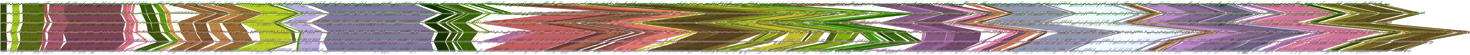
\includegraphics[width=1\textwidth]{images/collinear_zeae}  
  \end{center}
  When we compare two features (e.g. genes) between two or more genomes, there must be some basis for making the comparison \\
  That is, they have to be \textit{equivalent} in some way, such as:
  \begin{itemize}
    \item common evolutionary origin
    \item functional similarity
    \item a family-based relationship
  \end{itemize}
  It's common to define equivalence of genome features in terms of evolutionary relationship.
\end{frame}

% What do you align, and why?
\begin{frame}
  \frametitle{Why look at equivalent features?}
  \begin{center}
    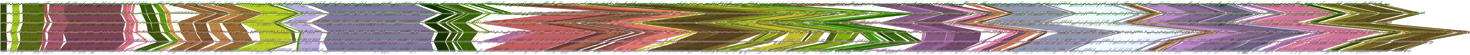
\includegraphics[width=1\textwidth]{images/collinear_zeae}  
  \end{center}
  \textbf{The real power of genomics is comparative genomics!}
  \begin{itemize}
    \item Makes catalogues of genome components comparable between organisms
    \item Differences, e.g. presence/absence of equivalents may support hypotheses for functional or phenotypic difference
    \item Can identify characteristic signals for diagnosis/epidemiology
    \item Can build parts lists and wiring diagrams for systems and synthetic biology
  \end{itemize}
\end{frame}
